\documentclass{zkdl-presentation-template}

\title[zk-SNARK I]{\textbf{QAP, PCP, POE}}
\author{Distributed Lab}
\date{Oct 1, 2024}
\titlegraphic{
    
\includegraphics[width=\textwidth]{images/banner_wide.png}
}

\begin{document}
    \frame {
        \titlepage
    }

    \begin{frame}{Plan}
        \tableofcontents
    \end{frame}

    \section{Recap}

    \begin{frame}{Recap. ZK-SNARK}
        \begin{definition}
            \textbf{zk-SNARK} – Zero-Knowledge Succinct Non-interactive ARgument of 
            Knowledge.
        \end{definition}
        \pause
        \begin{itemize}[itemsep=1pt]
            \item \textbf{Argument of Knowledge} --- a proof that the prover knows the data (witness) that resolves a certain
            problem, and this knowledge can be ``extracted''. \pause
            \item \textbf{Succinctness} --- the proof size and verification time is relatively small to the computation size and typically does not depend on the size of 
            the data or statement. \pause
            \item \textbf{Non-interactiveness} --- to produce the proof, the prover does not need any interaction
            with the verifier. \pause
            \item \textbf{Zero-Knowledge} --- the verifier learns nothing about the data used to produce the
            proof, despite knowing that this data resolves the given problem and that the prover possesses it.
        \end{itemize}
    \end{frame}

    \begin{frame}{Recap. Arbitrary Program To Circuits}
        We can do that in a way like the computer does it - boolean circuits.

        % --- Writing diagrams ---
        % Define circle styles and colors
        \colorlet{circle edge}{gray!50!black}
        \colorlet{circle area}{gray!20}
        \colorlet{gate1 edge}{green!50!black}
        \colorlet{gate1 area}{green!20}
        \colorlet{gate2 edge}{orange!50!black}
        \colorlet{gate2 area}{orange!20}
        \colorlet{gate3 edge}{blue!50!black}
        \colorlet{gate3 area}{blue!20}

        \tikzset{
            var/.style={circle, draw=circle edge, fill=circle area, very thick, minimum size=0.7cm, text centered},
            gate1/.style={circle, draw=gate1 edge, fill=gate1 area, ultra thick, minimum size=1cm, text centered},
            gate2/.style={circle, draw=gate2 edge, fill=gate2 area, ultra thick, minimum size=1cm, text centered},
            gate3/.style={circle, draw=gate3 edge, fill=gate3 area, ultra thick, minimum size=1cm, text centered},
            arrow/.style={-latex, ultra thick}
        }

        \begin{figure}[h!]
            \centering
            
            \begin{minipage}{0.54\textwidth}
                \centering
                % Boolean AND and OR gates
                \begin{tabular}{cc}
                    \begin{tikzpicture}
                        % Nodes
                        \node[var] (a) at (0, -1.5) {$a$};
                        \node[var] (b) at (2, -1.5) {$b$};
                        \node[gate1] (and) at (1, 0) {\texttt{AND}};
                        \node[var] (c) at (1, 1.75) {$c$};
        
                        % Arrows
                        \draw[arrow,gray] (a) -- (and);
                        \draw[arrow,gray] (b) -- (and);
                        \draw[arrow,gray!50!black] (and) -- (c);
                    \end{tikzpicture}
                    &
                    \begin{tikzpicture}
                        % Nodes
                        \node[var] (a) at (0, -1.5) {$a$};
                        \node[var] (b) at (2, -1.5) {$b$};
                        \node[gate2] (or) at (1, 0) {\texttt{OR}};
                        \node[var] (c) at (1, 1.75) {$c$};
        
                        % Arrows
                        \draw[arrow,gray] (a) -- (or);
                        \draw[arrow,gray] (b) -- (or);
                        \draw[arrow,gray!50!black] (or) -- (c);
                    \end{tikzpicture}
                \end{tabular}
                \centering
                \caption{Boolean \texttt{AND} and \texttt{OR} Gates}
            \end{minipage}
            \hspace{0.05\textwidth} % Space between figures
        \end{figure}

        But nothing stops us from using something more powerful instead of boolean values...
    \end{frame}

    \begin{frame}{Recap. Arbitrary Program To Circuits}
        We can do that in a way like the computer does it - boolean circuits.

        % --- Writing diagrams ---
        % Define circle styles and colors
        \colorlet{circle edge}{gray!50!black}
        \colorlet{circle area}{gray!20}
        \colorlet{gate1 edge}{green!50!black}
        \colorlet{gate1 area}{green!20}
        \colorlet{gate2 edge}{orange!50!black}
        \colorlet{gate2 area}{orange!20}
        \colorlet{gate3 edge}{blue!50!black}
        \colorlet{gate3 area}{blue!20}

        \tikzset{
            var/.style={circle, draw=circle edge, fill=circle area, very thick, minimum size=0.7cm, text centered},
            gate1/.style={circle, draw=gate1 edge, fill=gate1 area, ultra thick, minimum size=1cm, text centered},
            gate2/.style={circle, draw=gate2 edge, fill=gate2 area, ultra thick, minimum size=1cm, text centered},
            gate3/.style={circle, draw=gate3 edge, fill=gate3 area, ultra thick, minimum size=1cm, text centered},
            arrow/.style={-latex, ultra thick}
        }

        \begin{figure}[h!]
            \centering
            
            \begin{minipage}{0.54\textwidth}
                \centering
                % Boolean AND and OR gates
                \begin{tabular}{cc}
                    \begin{tikzpicture}
                        % Nodes
                        \node[var] (a) at (0, -1.5) {$a$};
                        \node[var] (b) at (2, -1.5) {$b$};
                        \node[gate1] (and) at (1, 0) {\texttt{AND}};
                        \node[var] (c) at (1, 1.75) {$c$};
        
                        % Arrows
                        \draw[arrow,gray] (a) -- (and);
                        \draw[arrow,gray] (b) -- (and);
                        \draw[arrow,gray!50!black] (and) -- (c);
                    \end{tikzpicture}
                    &
                    \begin{tikzpicture}
                        % Nodes
                        \node[var] (a) at (0, -1.5) {$a$};
                        \node[var] (b) at (2, -1.5) {$b$};
                        \node[gate2] (or) at (1, 0) {\texttt{OR}};
                        \node[var] (c) at (1, 1.75) {$c$};
        
                        % Arrows
                        \draw[arrow,gray] (a) -- (or);
                        \draw[arrow,gray] (b) -- (or);
                        \draw[arrow,gray!50!black] (or) -- (c);
                    \end{tikzpicture}
                \end{tabular}
                \centering
                \caption{Boolean \texttt{AND} and \texttt{OR} Gates}
            \end{minipage}
            \hspace{0.05\textwidth} % Space between figures
        \end{figure}
        > 100000 gates just for SHA256...
        \pause
        But nothing stops us from using something more powerful instead of boolean values, gates.
    \end{frame}

    \begin{frame}{Recap. Arbitrary Program To Circuits}
        Similar to Boolean Circuits, the \textbf{Arithmetic circuits} consist of gates and
        wires. 
        \begin{itemize}
            \item Wires: elements of some finite field $\mathbb{F}_p$.
            \item Gates: addition ($\oplus$) and multiplication ($\odot$) corresponding to the field.
        \end{itemize} 

        % --- Writing diagrams ---
        % Define circle styles and colors
        \colorlet{circle edge}{gray!50!black}
        \colorlet{circle area}{gray!20}
        \colorlet{gate1 edge}{green!50!black}
        \colorlet{gate1 area}{green!20}
        \colorlet{gate2 edge}{orange!50!black}
        \colorlet{gate2 area}{orange!20}
        \colorlet{gate3 edge}{blue!50!black}
        \colorlet{gate3 area}{blue!20}

        \tikzset{
            var/.style={circle, draw=circle edge, fill=circle area, very thick, minimum size=0.7cm, text centered},
            gate1/.style={circle, draw=gate1 edge, fill=gate1 area, ultra thick, minimum size=1cm, text centered},
            gate2/.style={circle, draw=gate2 edge, fill=gate2 area, ultra thick, minimum size=1cm, text centered},
            gate3/.style={circle, draw=gate3 edge, fill=gate3 area, ultra thick, minimum size=1cm, text centered},
            arrow/.style={-latex, ultra thick}
        }

        \begin{figure}[h!]
            \centering
            % Addition and Multiplication gates
            \begin{tabular}{cc}
                \begin{tikzpicture}
                    % Nodes
                    \node[var] (a) at (0, -1.5) {$a$};
                    \node[var] (b) at (2, -1.5) {$b$};
                    \node[gate1] (add) at (1, 0) {$+$};
                    \node[var] (c) at (1, 1.75) {$c$};

                    % Arrows
                    \draw[arrow,gray] (a) -- (add);
                    \draw[arrow,gray] (b) -- (add);
                    \draw[arrow,gray!50!black] (add) -- (c);
                \end{tikzpicture}
                &
                \begin{tikzpicture}
                    % Nodes
                    \node[var] (a) at (0, -1.5) {$a$};
                    \node[var] (b) at (2, -1.5) {$b$};
                    \node[gate2] (mul) at (1, 0) {$\times$};
                    \node[var] (c) at (1, 1.75) {$c$};

                    % Arrows
                    \draw[arrow,gray] (a) -- (mul);
                    \draw[arrow,gray] (b) -- (mul);
                    \draw[arrow,gray!50!black] (mul) -- (c);
                \end{tikzpicture}
            \end{tabular}
            \caption{Addition and Multiplication Gates}
        \end{figure}
    \end{frame}

    \begin{frame}[fragile]{Recap. Arbitrary Program To Circuits}
        \begin{example}
            How can we translate \texttt{if} statements?
            \begin{lstlisting}[language=Python, numbers=none, autogobble=true, xleftmargin=8pt]
                def example(a: bool, b: F, c: F) -> F:
                    if a:
                        return b * c 
                    else:
                        return b + c
            \end{lstlisting}
            \pause
            We can transform such a function into the next expression:
            \vspace{-8pt}
            \begin{equation*}
                r = a \times (b \times c) + (1 - a) \times (b + c)    
                \vspace{-8pt}
            \end{equation*}
            \pause
            Corresponding equations for the circuit are:
            \vspace{-8pt}
            \begin{equation*}
                \begin{aligned}
                    r_1 &= b \times c, \quad &r_3 &= 1 - a, \quad &r_5 &= r_3 \times r_2 \\
                    r_2 &= b + c, \quad &r_4 &= a \times r_1, \quad &r &= r_4 + r_5
                \end{aligned}
            \end{equation*}
        \end{example}
    \end{frame}

    \begin{frame}{Recap. Arbitrary Program To Circuits}
         % Define circle styles and colors
         \colorlet{circle edge}{gray!50!black}
         \colorlet{circle area}{gray!20}
         \colorlet{gate1 edge}{green!50!black}
         \colorlet{gate1 area}{green!20}
         \colorlet{gate2 edge}{orange!50!black}
         \colorlet{gate2 area}{orange!20}
         \colorlet{gate3 edge}{blue!50!black}
         \colorlet{gate3 area}{blue!20}
 
         \tikzset{
             var/.style={circle, draw=circle edge, fill=circle area, very thick, minimum size=0.7cm, text centered},
             gate1/.style={circle, draw=gate1 edge, fill=gate1 area, ultra thick, minimum size=1cm, text centered},
             gate2/.style={circle, draw=gate2 edge, fill=gate2 area, ultra thick, minimum size=1cm, text centered},
             gate3/.style={circle, draw=gate3 edge, fill=gate3 area, ultra thick, minimum size=1cm, text centered},
             arrow/.style={-latex, ultra thick}
         }
 
         \begin{figure}[h!]
             \centering
             \begin{tikzpicture}
                 % Nodes
                 \node[var] (c) at (0.5, -3) {$c$};
                 \node[var] (b) at (0.5, -1.5) {$b$};
                 \node[var] (a) at (0.5, 0) {$a$};
                 \node[var] (one) at (0.5, 1.5) {$1$};
         
                 % b+c and b*c gates
                 \node[gate1] (b_plus_c) at (2.5, -1.5) {$+$};
                 \node[gate2] (b_times_c) at (2.5, -3.0) {$\times$};
         
                 \node[gate3] (one_minus_a) at (2.5, 0.75) {$-$};
         
                 % a*b*c and (1-a)(b+c) gates
                 \node[gate2] (a_times_b_times_c) at (5, -2.0) {$\times$};
                 \node[gate2] (one_minus_a_times_b_plus_c) at (5, -0.5) {$\times$};
         
                 % a*b*c + (1-a)(b+c) gate
                 \node[gate1] (r) at (7.5, -1.25) {$+$};
         
                 % Result node
                 \node[var] (result) at (10, -1.25) {$r$};
         
                 % b+c and b*c arrows
                 \draw[arrow,gray] (b) to (b_plus_c);
                 \draw[arrow,gray] (b) to (b_times_c);
                 \draw[arrow,gray] (c) to (b_plus_c);
                 \draw[arrow,gray] (c) to (b_times_c);
         
                 % 1 - c arrow
                 \draw[arrow,gray] (one) to (one_minus_a);
                 \draw[arrow,gray] (a) to (one_minus_a);
         
                 % a*b*c and (1-a)(b+c) arrows
                 \draw[arrow,gray] (a) to [bend left=20] (a_times_b_times_c);
                 \draw[arrow,gray] (b_times_c) to node[midway, above] {$r_1$} (a_times_b_times_c);
                 \draw[arrow,gray] (one_minus_a) to node[midway, above] {$r_3$} (one_minus_a_times_b_plus_c);
                 \draw[arrow,gray] (b_plus_c) to node[midway, above] {$r_2$} (one_minus_a_times_b_plus_c);
         
                 % a*b*c + (1-a)(b+c) arrows
                 \draw[arrow,gray] (a_times_b_times_c) to [bend right=20] node[midway, above] {$r_4$} (r);
                 \draw[arrow,gray] (one_minus_a_times_b_plus_c) to [bend left=20] node[midway, above] {$r_5$} (r);
         
                 % Result arrow
                 \draw[arrow,gray!50!black] (r) to (result);
         
             \end{tikzpicture}
             \caption{Example of a circuit evaluating the \texttt{if} statement logic.}
             \label{fig:multivariate-polynomial-circuit}
         \end{figure}
    \end{frame}

    \begin{frame}[fragile]{Recap. Arbitrary Program To Circuits}
        \begin{example}
            How can we translate \texttt{if} statements?
            \begin{lstlisting}[language=Python, numbers=none, autogobble=true, xleftmargin=8pt]
                def example(a: bool, b: F, c: F) -> F:
                    if a:
                        return b * c 
                    else:
                        return b + c
            \end{lstlisting}
            \pause
            We can transform such a function into the next expression:
            \vspace{-8pt}
            \begin{equation*}
                r = a \times (b \times c) + (1 - a) \times (b + c)    
                \vspace{-8pt}
            \end{equation*}
            \pause
            Corresponding equations for the circuit are:
            \vspace{-8pt}
            \begin{equation*}
                \begin{aligned}
                    r_1 &= b \times c, \quad &r_3 &= 1 - a, \quad &r_5 &= r_3 \times r_2 \\
                    r_2 &= b + c, \quad &r_4 &= a \times r_1, \quad &r &= r_4 + r_5
                \end{aligned}
            \end{equation*}
        \end{example}
    \end{frame}

    \begin{frame}{Recap. R1CS}
        Each \textbf{constraint} in the Rank-1 Constraint System must be in the form:
        \begin{equation*}
            \langle \mathbf{a}, \mathbf{w}\rangle \times \langle \mathbf{b}, \mathbf{w}\rangle = \langle \mathbf{c}, \mathbf{w}\rangle
        \end{equation*}
        \pause
        Where $\langle \mathbf{u}, \mathbf{v}\rangle$ is a dot product.
        \vspace{-10pt}
        \begin{equation*}
            \langle \mathbf{u}, \mathbf{v} \rangle := \mathbf{u}^{\top}\mathbf{v} = \sum_{i=1}^{n} u_i v_i 
            \vspace{-5pt}
        \end{equation*}
        \pause
        Thus
        \vspace{-5pt}
        \begin{equation*}
            \left(\sum_{i=1}^{n} a_i w_i\right) \times \left(\sum_{j=1}^{n} b_j w_j\right) = \sum_{k=1}^{n} c_k w_k
        \end{equation*}
        That is, actually, a quadratic equation with multiple variables.
    \end{frame}

    \begin{frame}{Recap. R1CS}
        \begin{example}
            Consider the most basic circuit with one multiplication gate: $x_1 \times x_2 = r$.
            The witnes vector $\mathbf{w} = (r, x_1, x_2)$. So
            \vspace{-5pt}
            \begin{align*}
                w_2 &\times w_3 = w_1 \\
                (0 + w_2 + 0) &\times (0 + 0 + w_3) = w1 + 0 + 0 \\
                (0w_1 + 1w_2 + 0w_3) &\times (0w_1 + 0w_2 + 1w_3) = 1w_1 + 0w_2 + 0w_3
            \end{align*}
            Therefore the coefficients vectors are:
            \vspace{-5pt}
            \begin{equation*}
                \mathbf{a} = (0, 1, 0), \quad \mathbf{b} = (0, 0, 1), \quad \mathbf{c} = (1, 0, 0). 
                \vspace{-5pt}
            \end{equation*}
            The general form of our constraint is:
            \vspace{-5pt}
            \begin{equation*}
                (a_1w_1 + a_2w_2 + a_3w_3)(b_1w_1 + b_2w_2 + b_3w_3) = c_1w_1 + c_2w_2 + c_3w_3
            \end{equation*}
        \end{example}
    \end{frame}

    \begin{frame}{Recap. R1CS}
        \vspace{-10pt}
        \begin{equation*}
            r = x_1 \times (x_2 \times x_3) + (1 - x_1) \times (x_2 + x_3)
        \end{equation*}
        \pause
        Thus, the next constraints can be build:
        \vspace{-5pt}
        \begin{align*}
            x_1 \times x_1 &= x_1 \quad \text{(binary check)} \tag{1} \\
            x_2 \times x_3 &= \mathsf{mult} \tag{2} \\
            x_1 \times \mathsf{mult} &= \mathsf{selectMult} \tag{3} \\
            (1 - x_1) \times (x_2 + x_3) &= r - \mathsf{selectMult} \tag{4}
        \end{align*}
        \pause
        The witness vector: $\mathbf{w} = (1, r, x_1, x_2, x_3, \mathsf{mult}, \mathsf{selectMult})$.
        
        \pause
        \vspace{2pt}
        The coefficients vectors:
        \vspace{-25pt}
        {\center\small\begin{align*}
            \mathbf{a}_1 &= (0, 0, 1, 0, 0, 0, 0), & \mathbf{b}_1 &= (0, 0, 1, 0, 0, 0, 0), & \mathbf{c}_1 &= (0, 0, 1, 0, 0, 0, 0) \\
            \mathbf{a}_2 &= (0, 0, 0, 1, 0, 0, 0), & \mathbf{b}_2 &= (0, 0, 0, 0, 1, 0, 0), & \mathbf{c}_2 &= (0, 0, 0, 0, 0, 1, 0) \\
            \mathbf{a}_3 &= (0, 0, 1, 0, 0, 0, 0), & \mathbf{b}_3 &= (0, 0, 0, 0, 0, 1, 0), & \mathbf{c}_3 &= (0, 0, 0, 0, 0, 0, 1) \\
            \mathbf{a}_4 &= (1, 0, -1, 0, 0, 0, 0), & \mathbf{b}_4 &= (0, 0, 0, 1, 1, 0, 0), & \mathbf{c}_4 &= (0, 1, 0, 0, 0, 0, -1)
        \end{align*}}
    \end{frame}
    
    \section{Quadratic Arithmetic Program}

    \begin{frame}
        Problems we have for now: \pause
        \begin{itemize}
            \item Although Rank-1 Constraint Systems provide a powerful method for representing 
            computations, they are not succinct. \pause
            \item We need to transform our computations into a form that is more convenient for 
            proving statements about them.
        \end{itemize}
    \end{frame}

    \begin{frame}
        We finished with:
        \begin{equation*}
            \mathbf{a_1}, \mathbf{a_2}, \dots, \mathbf{a_m}, \quad
            \mathbf{b_1}, \mathbf{b_2}, \dots, \mathbf{b_m}, \quad
            \mathbf{c_1}, \mathbf{c_2}, \dots, \mathbf{c_m}, 
        \end{equation*}
        \pause
        Of course, they form corresponding matrices:
        {\scriptsize \begin{align*}
            A = \begin{bmatrix}
                a_{11} & a_{12} & \dots & a_{1n} \\
                a_{21} & a_{22} & \dots & a_{2n} \\
                \vdots & \vdots & \ddots & \vdots \\
                a_{m1} & a_{m2} & \dots & a_{mn}
            \end{bmatrix} & \quad
            B = \begin{bmatrix}
                b_{11} & b_{12} & \dots & b_{1n} \\
                b_{21} & b_{22} & \dots & b_{2n} \\
                \vdots & \vdots & \ddots & \vdots \\
                b_{m1} & b_{m2} & \dots & b_{mn}
            \end{bmatrix} & 
            C = \begin{bmatrix}
                c_{11} & c_{12} & \dots & c_{1n} \\
                c_{21} & c_{22} & \dots & c_{2n} \\
                \vdots & \vdots & \ddots & \vdots \\
                c_{m1} & c_{m2} & \dots & c_{mn}
            \end{bmatrix}
        \end{align*}}
        \pause
        An example of a single ``if`` statement:
        \begin{center}
        \begin{minipage}{0.4\textwidth}
        \vspace{-15pt}
        {\scriptsize \begin{align*}
            \mathbf{a}_1 &= (0, 0, 1, 0, 0, 0, 0) \\
            \mathbf{a}_2 &= (0, 0, 0, 1, 0, 0, 0) \\
            \mathbf{a}_3 &= (0, 0, 1, 0, 0, 0, 0) \\
            \mathbf{a}_4 &= (1, 0, -1, 0, 0, 0, 0)
        \end{align*}}
        \end{minipage}
        \begin{minipage}{0.5\textwidth}
        \begin{tikzpicture}
            \node (A) at (0,0) {$
                A = {\scriptsize \begin{bmatrix}
                    0 & 0 & 1 & 0 & 0 & 0 & 0 \\
                    0 & 0 & 0 & 1 & 0 & 0 & 0 \\
                    0 & 0 & 1 & 0 & 0 & 0 & 0 \\
                    1 & 0 & -1 & 0 & 0 & 0 & 0 \\
                \end{bmatrix}}
            $};
        \end{tikzpicture}
        \end{minipage}
        \end{center}
            
        \pause
        Pleeeeeenty of zeroes, doesn't it? And this is just one out of 3 matrices...
    \end{frame}

    \begin{frame}
        The previous witness vector:
        \vspace{-10pt}
        \begin{center}
            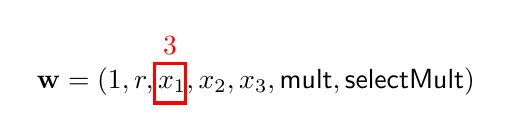
\begin{tikzpicture}
                % Node to contain the pmatrix
                \node (A) at (0,0) {$\mathbf{w} = (1, r, x_1, x_2, x_3, \mathsf{mult}, \mathsf{selectMult})$};
            
                \pause
                % Draw the red rectangle around the third column
                \draw[red, very thick] 
                    ([xshift=-108pt,yshift=-2pt]A.north east) -- ++(0,-0.5) -- 
                    ++(-0.4,0) -- ++(0,0.5) -- cycle;

                \node[xshift=-31pt,yshift=13pt,text=red] (B) at (0,0) {3};
            \end{tikzpicture}
        \end{center}
        \vspace{-8pt}
        Let's take a closer look at the matrix columns:
        \vspace{-8pt}
        \begin{center}
            \begin{tikzpicture}
                % Node to contain the pmatrix
                \node (A) at (0,0) {$
                    \begin{bmatrix}
                        0 & 0 & 1 & 0 & 0 & 0 & 0 \\
                        0 & 0 & 0 & 1 & 0 & 0 & 0 \\
                        0 & 0 & 1 & 0 & 0 & 0 & 0 \\
                        1 & 0 & -1 & 0 & 0 & 0 & 0 \\
                    \end{bmatrix}
                $};
            
                % Draw the red rectangle around the third column
                \draw[red, very thick] 
                    ([xshift=-71pt,yshift=-2pt]A.north east) -- ++(0,-1.93) -- 
                    ++(-0.7,0) -- ++(0,1.93) -- cycle;

                \node[xshift=-16pt,yshift=35pt,text=red] (B) at (0,0) {3};
            \end{tikzpicture}
        \end{center}
        \vspace{-10pt}
        Consider 4th constraint: $(1 - x_1) \times (x_2 + x_3) = r - \mathsf{selectMult}$
        \vspace{-8pt}
        \begin{center}
            \begin{tikzpicture}
                % Node to contain the pmatrix
                \node (A) at (0,0) {$
                    \begin{bmatrix}
                        0 & 0 & 1 & 0 & 0 & 0 & 0 \\
                        0 & 0 & 0 & 1 & 0 & 0 & 0 \\
                        0 & 0 & 1 & 0 & 0 & 0 & 0 \\
                        1 & 0 & -1 & 0 & 0 & 0 & 0 \\
                    \end{bmatrix}
                $};
            
                % Draw the red rectangle around the third column
                \draw[red, very thick] 
                    ([xshift=-71pt,yshift=-2pt]A.north east) -- ++(0,-1.93) -- 
                    ++(-0.7,0) -- ++(0,1.93) -- cycle;

                \node[xshift=-16pt,yshift=35pt,text=red] (B) at (0,0) {3};

                \draw[blue!70!black, very thick] 
                    ([xshift=-7.75pt,yshift=-45pt]A.north east) -- ++(-4,0) -- 
                    ++(0,-0.42) -- ++(4,0) -- cycle;
    
                \node[xshift=-63pt,yshift=-20pt,text=blue!70!black] (B) at (0,0) {4};

                \draw[black, very thick] 
                    ([xshift=-71pt,yshift=-45pt]A.north east) -- ++(-0.7,0) -- 
                    ++(0,-0.42) -- ++(0.7,0) -- cycle;
            \end{tikzpicture}
        \end{center}
        \pause
        \vspace{-10pt}
        So, every column is a mapping of constraint number to a coefficient for the witness element.
    \end{frame}

    \begin{frame}
        As we know, such a mapping can be builds using Lagrange interpolation polynomial with the
        following formula:
        \vspace{-10pt}
        \begin{equation*}
            L(x) = \sum_{i=0}^{n} y_i \ell_i(x), \quad \ell_i(x) = \prod_{j=0, j \neq i}^{n} \frac{x-x_j}{x_i-x_j}.
            \vspace{-10pt}
        \end{equation*}  

        \pause
        There are $n$ columns and $m$ constraints. So, it results in $n$ polynomials such that:
        \vspace{-10pt}
        \begin{equation*}
            A_j(i) = a_{i,j}, \; i \in \{1,2,\dots,m\}, \; j \in \{1,2,\dots,n\}
            \vspace{-10pt}
        \end{equation*}

        \pause
        The same is true for matrices $B$ and $C$, with $3n$ polynomials in total, $n$ for each of the
        coefficients matrices:
        \vspace{-8pt}
        \begin{align*}
            A_1(x), A_2(x), \dots, A_n(x), 
            B_1(x), B_2(x), \dots, B_n(x),
            C_1(x), C_2(x), \dots, C_n(x)
            \vspace{-10pt}
        \end{align*}

        \vspace{-10pt}
        \pause
        \begin{block}{Note}
            We could have assigned any \textit{unique} index from $\mathbb{F}$ to each constraint
            (say, $t_i$ for each $i \in \{1,\dots,m\}$) and interpolate through these points:
            \vspace{-8pt}
            \begin{equation*}
                A_j(t_i) = a_{i,j}, \; i \in \{1,2,\dots,m\}, \; j \in \{1,2,\dots,n\}
            \end{equation*}
        \end{block}
    \end{frame}

    \begin{frame}{}
        \centering \Large
        \emph{Thanks for your attention!}
    \end{frame}
\end{document}